% example.tex
\documentclass[dvisvgm]{standalone}

\usepackage{amsmath}
\usepackage[usenames,dvipsnames]{xcolor}
\usepackage{amsmath}
\usepackage{tikz}
\usetikzlibrary {angles,
                 arrows.meta,
                 calc,
                 positioning,
                 shapes.geometric}

 \tikzset{
        square/.style={regular polygon, regular polygon sides=4},
        base/.style={draw, align=center, minimum height=4ex},
        proc/.style={base, rectangle, text width=8em},
        io/.style={trapezium, trapezium left angle=70, trapezium right
                   angle=110, draw, text width=8em, %minimum width=2cm, 
                   %minimum height=1cm
                   },
        test/.style={base, diamond, aspect=2,
                     %text width=5em
                     },
        term/.style={proc, rounded corners},
        myarrow/.style={-Stealth, line width=0.25mm},
 }

\begin{document}
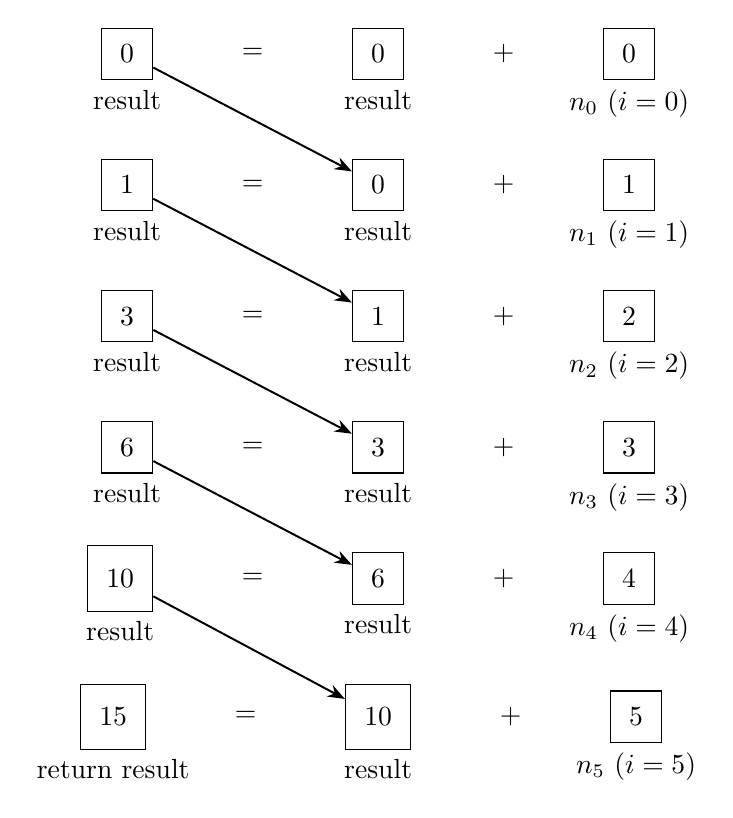
\begin{tikzpicture}
    \node[draw, square, label=below: result] (a) {0};
    \node[right= of a] (b) {$+$};
    \node[draw, square, right=of b, label=below:{$n_0\ (i=0)$}] (c) {0};
    \node[left= of a] (1a) {$=$};
    \node[draw, square, left=of 1a, label=below: result] (0a) {0};

    \node[draw, square, below= of a, label=below: result] (a1) {0};
    \node[right= of a1] (b1) {$+$};
    \node[draw, square, right=of b1, label=below:{$n_1\ (i=1)$}] (c1) {1};
    \node[left= of a1] (1a1) {$=$};
    \node[draw, square, left=of 1a1, label=below: result] (0a1) {1};

    \node[draw, square, below= of a1, label=below: result] (a2) {1};
    \node[right= of a2] (b2) {$+$};
    \node[draw, square, right=of b2, label=below:{$n_2\ (i=2)$}] (c2) {2};
    \node[left= of a2] (1a2) {$=$};
    \node[draw, square, left=of 1a2, label=below: result] (0a2) {3};

    \node[draw, square, below= of a2, label=below: result] (a3) {3};
    \node[right= of a3] (b3) {$+$};
    \node[draw, square, right=of b3, label=below:{$n_3\ (i=3)$}] (c3) {3};
    \node[left= of a3] (1a3) {$=$};
    \node[draw, square, left=of 1a3, label=below: result] (0a3) {6};

    \node[draw, square, below= of a3, label=below: result] (a4) {6};
    \node[right= of a4] (b4) {$+$};
    \node[draw, square, right=of b4, label=below:{$n_4\ (i=4)$}] (c4) {4};
    \node[left= of a4] (1a4) {$=$};
    \node[draw, square, left=of 1a4, label=below: result] (0a4) {10};

    \node[draw, square, below= of a4, label=below: result] (a5) {10};
    \node[right= of a5] (b5) {$+$};
    \node[draw, square, right=of b5, label=below:{$n_5\ (i=5)$}] (c5) {5};
    \node[left= of a5] (1a5) {$=$};
    \node[draw, square, left=of 1a5, label=below: return result] (0a5) {15};


    \draw[myarrow] (0a) -- (a1);
    \draw[myarrow] (0a1) -- (a2);
    \draw[myarrow] (0a2) -- (a3);
    \draw[myarrow] (0a3) -- (a4);
    \draw[myarrow] (0a4) -- (a5);
\end{tikzpicture}
\end{document}
